\section{Marco Teórico}
\subsection{Definiciones}
\begin{itemize}
    \item \textbf{Nave perseguidora}: nave que realiza los impulsos y busca interceptar a los dos objetos.
\end{itemize}

\subsection{Conceptos}
El problema de interceptación de dos objetivos con un solo
impulso es un reto fundamental en la mecánica orbital, particularmente en las
misiones espaciales que requieren la optimización de maniobras para
minimizar el uso de combustible \parencite{Battin1999}.
\subsubsection{Interceptación Orbital}
La interceptación orbital es el proceso
mediante el cual una nave espacial ajusta su trayectoria para alcanzar
un objetivo en el espacio.
\subsubsection{Two-Body Model}
El modelo de dos cuerpos es un modelo simplificado en mecánica orbital
que describe el movimiento (elíptico) de dos cuerpos bajo la influencia
mutua de la gravedad, sin tener en cuenta otras fuerzas externas (como las
perturbaciones atmosféricas) \parencite{Cerf2013}.
\subsubsection{Impulso}
En astrodinámica, el impulso es un cambio abrupto en la
velocidad de una nave espacial, que altera su trayectoria orbital.
\subsubsection{Transferencia}
Las transferencias elípticas
son trayectorias cerradas en forma de elipse, mientras que las
transferencias hiperbólicas son trayectorias abiertas que permiten a
un objeto escapar de la atracción de un cuerpo central (como la
Tierra) \parencite{ZHU20162177}.
\subsubsection{Perturbación J2}
La perturbación J2 es el efecto causado por la
forma no esférica de la Tierra, que altera ligeramente las órbitas de
los objetos cercanos debido a la asimetría gravitacional de la Tierra
(concentrada en el ecuador).
%
\subsection{Métodos Numéricos}
\subsubsection{Gráfico Porkchop}
Este método se utiliza para visualizar las posibles combinaciones de
los tiempos de impulso $t_0$ y tiempos de intercepción $t_1$ que minimizan
el tiempo total de la misión o el uso de combustible \parencite{DUAN2020965}.

El gráfico de Porkchop calcula el coste asociado a cada combinación
de $t_0$ y $t_1$ mediante una fórmula de la forma:

\begin{equation}
    \begin{split}
        P(t_0, t_1) = \left| t_1 - t_0 - \frac{M_3(t_1) - M_3(t_0)}{n_3} \right| \\
        + \left| t_2 - t_0 - \frac{M_3(t_2) - M_3(t_0)}{n_3} \right|
    \end{split}
\end{equation}


\begin{itemize}
    \item $M_3(t)$: anomalía media en el tiempo $t$.
    \item $n_3$: movimiento medio de la órbita de la nave perseguidora.
    \item $t_2$: tiempo de intercepción con el segundo objetivo.
\end{itemize}

\begin{center}
    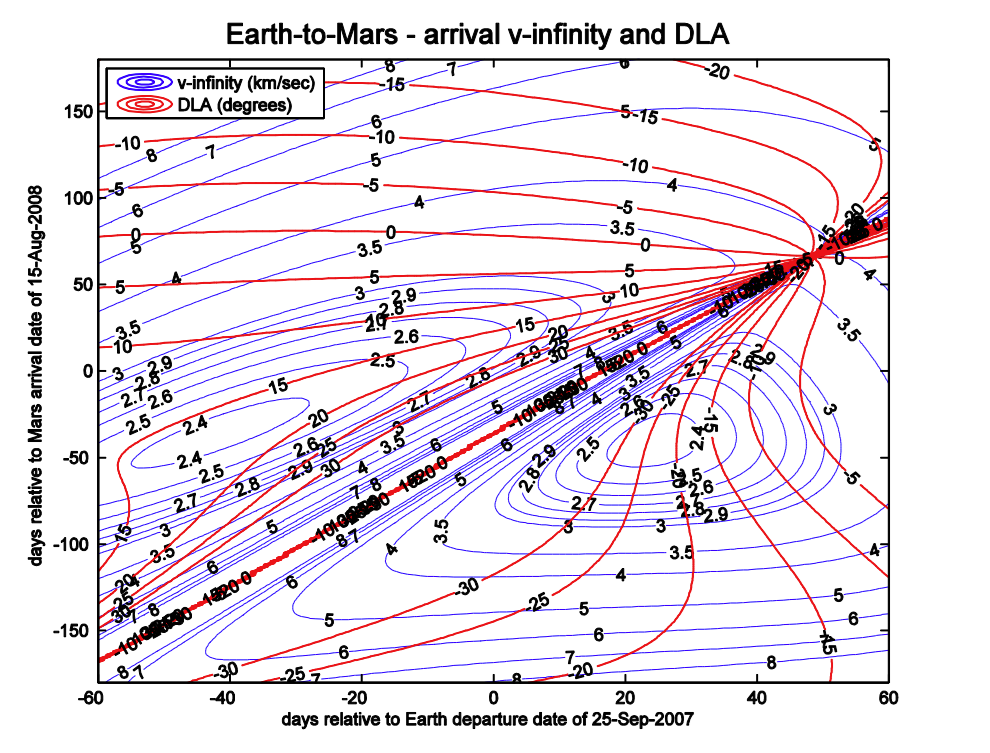
\includegraphics[width=0.4\textwidth]{porkchop_ejemplo.png}
    \captionof{figure}{Ejemplo de Porkchop plot.} \parencite{eagle2025}
\end{center}

\subsubsection{Método de Gibbs}
Una vez que se
han obtenido las estimaciones iniciales de $t_0$ y $t_1$ a partir del gráfico
Porkchop, se utiliza el Método de Gibbs para determinar la órbita
de la nave perseguidora. Gracias a esto, se reduce la cantidad de variables independientes
de seis a dos. Este concepto se explica más a profundidad en la sección de formulación del problema.

El método de Gibbs calcula la velocidad orbital de
la nave a partir de tres vectores de posición conocidos de la nave y
los dos objetivos \parencite{HE2010265}. A partir de los tres
vectores de posición $r_1$, $r_2$ y $r_3$, se calcula la velocidad de la nave
perseguidora en la órbita de intercepción con la siguiente fórmula:

\begin{equation}
    v_{3,tk} = \sqrt{\frac{\mu}{ND} \left( \frac{D \ast r_{3,tk}}{r_{3,tk}} + S \right)}
\end{equation}

Donde:
\begin{itemize}
    \item $v_{3,tk}$: vector de velocidad de la nave perseguidora en el tiempo $t_k$.
    \item $\mu$: constante gravitacional de la Tierra.
    \item N, D, y S\@: valores derivados del producto cruz entre los vectores de posición.
\end{itemize}

\subsubsection{Método de Newton-Raphson}
El Método de Newton-Raphson es un algoritmo iterativo utilizado para resolver sistemas de ecuaciones no lineales, y es esencial para refinar las soluciones obtenidas con los métodos anteriores.
En este caso, se utiliza para ajustar las variables $t_0$, $t_1$, $t_2$ y el vector de impulso $v$ hasta que se cumplan las condiciones de interceptación.

Fórmula de iteración:
\[
    x_{n+1} = x_n - J{(x_n)}^{-1} \ast F(x_n)
\]

Donde:
\begin{itemize}
    \item $x_n$ es el vector de valores actuales de las variables.
    \item $J$ es la matriz Jacobiana de las ecuaciones no lineales.
    \item $F(x_n)$ es el vector de funciones (las ecuaciones de las posiciones y tiempos de interceptación).
\end{itemize}
